\documentclass[12pt,letter,oneside]{report}
\usepackage{fullpage}
\usepackage{titlesec}
\usepackage{graphicx}
\usepackage{indentfirst}
\usepackage{siunitx}
\titleformat{\chapter}{\bf\Large}{\thechapter}{0.5em}{}
\titlespacing*{\chapter}{0pt}{-20pt}{20pt}
\titleformat{\section}{\bf\large}{\thesection}{0.2em}{}
\titleformat{\subsection}{\bf\normalsize}{\thesubsection}{0.1em}{}
\newcommand{\HRule}{\rule{\linewidth}{0.5mm}}
\newcommand{\superscript}[1]{\ensuremath{^{\textrm{#1}}}}
\newcommand{\multiline}[2][t]{\begin{tabular}[#1]{@{}l@{}}#2\end{tabular}}
\renewcommand{\chaptername}{}
%Uncomment the next line to supress numbering
%\renewcommand{\thechapter}{}
\begin{document}
\begin{titlepage}
\begin{center}

% Upper part of the page
\textsc{\Large Final Report}\\[0.5cm]


% Title
\HRule \\[0.4cm]
{ \huge \bfseries USB Data Logger}\\[0.4cm]

\HRule \\[1.5cm]

% Author and supervisor
\large
\emph{Authors:}\\
Spencer \textsc{Julian}\\
David \textsc{Kauer}\\
John \textsc{Wyant}\\
Jintao \textsc{Zhang}\\
\vfill
\large
\emph{Course:} \textsc{ECE 337}\\
\emph{Lab:} \textsc{Tuesday 2:30 - 5:30}\\
\emph{TA:} Tom \textsc{Pollard}

\vfill

% Bottom of the page
\large April 28, 2012
%{\large \today}

\end{center}

\end{titlepage}

\tableofcontents
\chapter{Executive Summary}
The team for this project successfully created an ASIC design that reads incoming data from a USB interface and stores the data onto a microSD card. The purpose of this device would be to gain potentially valuable information such as passwords, webcam discussions, typed documents, or debugging information. This makes the device particularly useful for certain tasks such as espionage, debugging a USB device, or ensuring that critical components properly communicate via USB. An important part of this device is that the connections are subtle and transparent in order to avoid disrupting the user and calling unwanted attention upon itself.

It also records all intercepted data to a microSD card, which allows the device to store a massive amount of data. The device records to a microSD card because it is a fast and easy method to collect data, and it allows for new data to be stored onto another microSD card when the original one is pulled out to examine data. The USB logger is designed to intercept any USB handshakes and convert them from USB 2.0 or USB 3.0 to a USB 1.1 connection. After converting the handshake, the data logger becomes transparent in the communication across the USB bus and begins to write the data passing through it onto the microSD card.

The remainder of this document describes the design specifications and the final architecture of the chip, which includes a functional block diagram. It will show the input and output pins on the chip, interfacing specifications, operational characteristics, and specific requirements necessary to run the device. This report will also describe the USB and microSD protocols involved in designing and testing, as well as the timing and area budgets of the USB logger. Finally, there is a description of the tests that are performed on the design as well as the results that can be taken from those tests, and a description of the chip layout. 
\chapter{Design Specifications}
\section{Interfacing Specifications}
\begin{figure}[h]
	\caption{The USB Data Logger Usage Digram. The central box is the device.}
	\begin{center}
		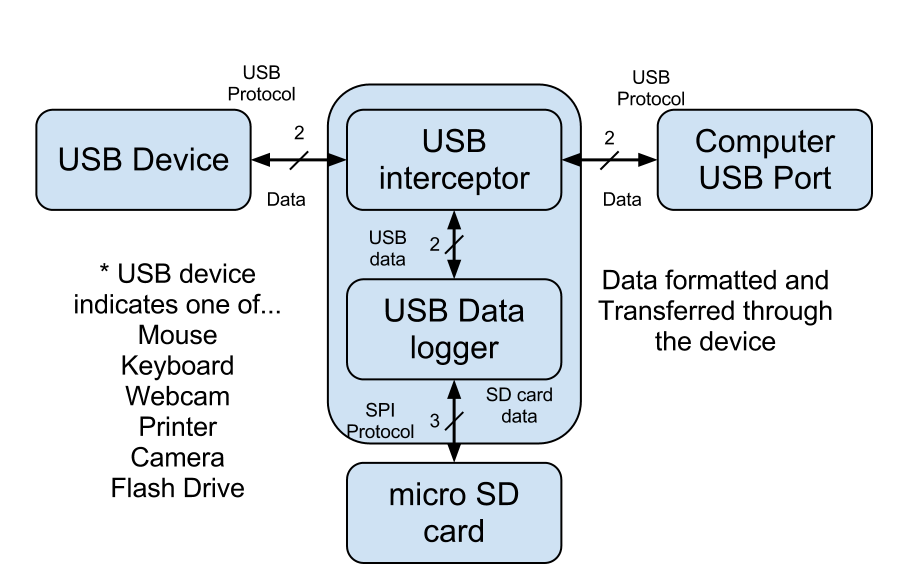
\includegraphics[width=0.85\textwidth]{usageDiagram}
	\end{center}
\end{figure}
The protocols used, as defined in figure 2.1, above, are:
\begin{description}
	\item[USB 1.1] \hfill \\
		Transmission rate of 12 Mbps.
	\item[SPI] \hfill \\
		Transmission rate of 50Mbps after initalization, 400kbps during initalization.
\end{description}
\pagebreak
\section{Operational Characteristics}
\subsection{Pin-out}
\begin{table}[h]
	\caption{The USB Data Logger Pin-Out table.}
	\centering
	\begin{tabular}{| l | l | p{1.5cm} | p{3cm} | p{4cm} |}
		\hline
		\bf{Signal Name} & \bf{Type} & \bf{Number of Bits} & \bf{Data Format} & \bf{Description and Timing Constraints} \\ \hline
		clk              & In        & 1                   & System Clock     & Clock signal for the chip               \\ \hline
		rst              & In        & 1                   & Active Low       & Asynchronous reset signal for the device's memory elements. \\ \hline
		PWR & In & 1 & Power & Power Input \\ \hline
		GND & In & 1 & Ground & Ground Line \\ \hline
		dataPlusUsb & Bidirectional & 1 & LSB NRZI & USB Data+ Line \\ \hline
		dataMinusUsb & Bidirectional & 1 & LSB NRZI, inverted Data+ Line, above & USB Data- Line \\ \hline
		dataPlusComputer & Bidirectional & 1 & LSB NRZI & Computer Data+ Line \\ \hline
		dataMinusComputer & Bidirectional & 1 & LSB NRZI, inverted Data+ Line, above & Computer Data- Line \\ \hline
		scl & Out & 1 & Clock & Clock output to microSD Card \\ \hline
		sd\_enable & Out & 1 & Active Low & Chip Select for microSD Card \\ \hline
		dataOut & Out & 1 & Active High Binary & MOSI Data Output to microSD Card \\ \hline
	\end{tabular}
\end{table}
\pagebreak
\subsection{Chip Operation Sequence}
\begin{figure}[h]
	\caption{A flowchart of the USB Data Logger's operation}
	\begin{center}
		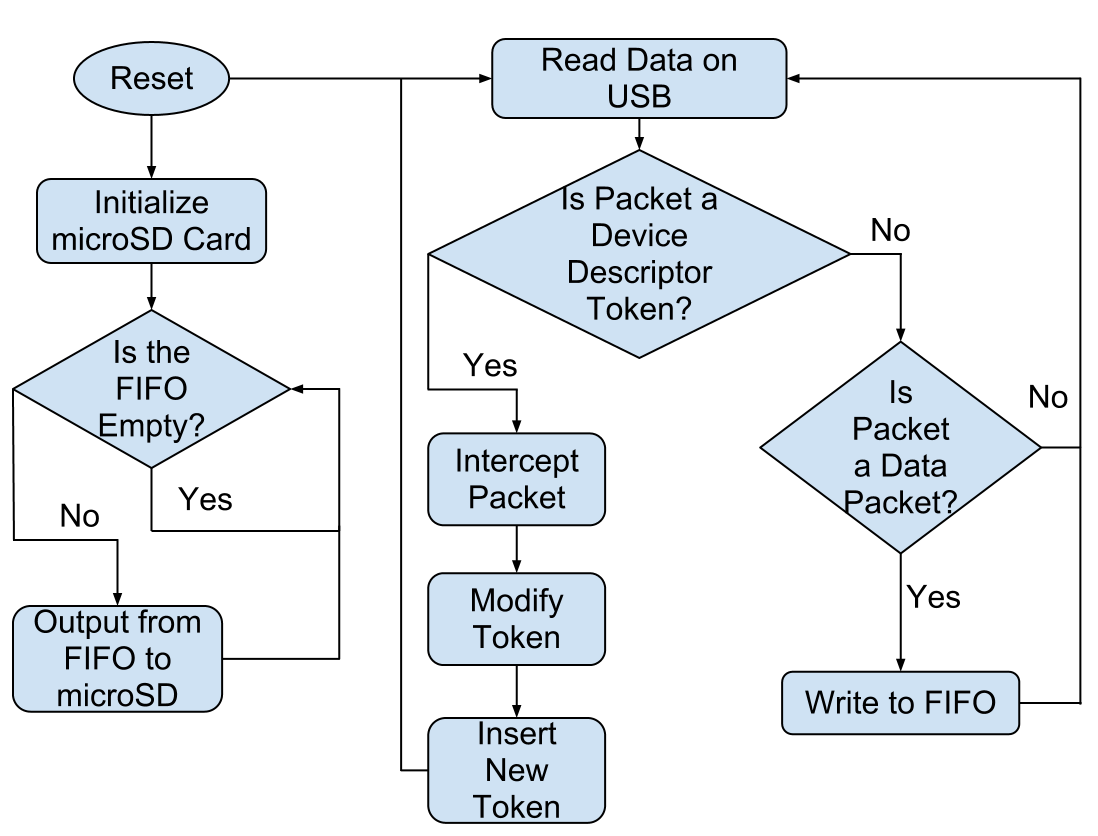
\includegraphics[width=0.85\textwidth]{OperationalTimeline}
	\end{center}
\end{figure}
\subsubsection{General Operation}
As shown in figure 2.2 above, the operation has two concurrent timelines operating after reset. The first timeline, shown as the left branch (going down from the reset block), is for the microSD card, and the second timeline (from the right of the reset block) is for USB communication.
\subsubsection{USB Operation}
As soon as the device resets, it begins listening on the USB line for any packet coming through. If the packet is a device descriptor token, identified by a specific PID, then it will intercept the packet and insert our modified description. It will only intercept the two relevant bytes to change the USB version number to USB 1.1, identified in hexidecimal, most significant bit first, as 0x0110. After it modifies the description, it injects it into the line, and the computer will read our modified description instead of the one sent by the device. This process delays the entire line slightly, but the delay is consistent, and remains even when the packet is not a device descriptor, so it will cause no errors in communication.

If the packet is a data packet, then it will write the data to an internal FIFO block where it will wait to be written to the microSD card. The device will only write data from the data packets, the rest of the packet will be ignored and discarded by the device for writing, though it will still pass through the device without issue to ensure proper operation of both connected devices.
\subsubsection{SD Operation}
When the device resets, the microSD card must be initialized. This is a relatively long process, as it takes one half of a millisecond. The card is initialized by waiting 80 clock cycles at \SI{400}{\kilo\hertz}, followed by outputting a command to switch it into SPI mode from SD mode and prepare for writing. Once the card is initialized we can speed up to the full \SI{50}{\mega\hertz} for writing.

Unfortunately, due to a limitation in the inital design of our device, we cannot listen for card responses via MISO. However, all tested cards have been shown to respond favorably within a limited period of time, so our commands wait for this period of time before continuing writes.

After the microSD card is initialized, we see if the FIFO is empty. If it is empty, the SD clock will not be running, and we will simply wait for data to enter the FIFO. If the FIFO is not empty, we will output each byte that is inside the FIFO until it is empty, where we will stop the SD clock and wait for more data.

After a CMD25, which is the continous write command, the SD protocol usually defines a stop bit to indicate when we are finished writing to the device. However, due to the continuous operation of our device with no appropriate "stop" signal, other than unplugging the device thus ceasing all operation, we have not implemented this stop signal. It should not be a concern as we are performing a bit-by-bit write via SPI instead of writing using the SD protocol.
\section{Requirements}
As the USB logger tricks the device that is plugged into it to use the USB 1.1 protocol, I/O speed and internal clock speed are not a big concern, as USB 1.1 runs at a speed of 12 Mbps. The device’s clock speed can run at \SI{140}{\mega\hertz}. Power is also not a big concern, since 5+ volts and ground are leeched from the USB, which should provide more than enough power for both our device as well as the device that is plugged into it. Therefore, area is our most critical design restriction.

The area of the chip must be small, as the entire device must not be larger than the size of a microSD card. If external storage was not necessary, it would be ideal to have a chip that could fit on a USB connector so that it would be very difficult to detect. As the primary use of this device will be for secretive data collecting, the harder it is to find, the better.

An added bonus of decreasing the size is decreasing power. While our power constraints are minimal, if we decrease power that will make it more difficult for someone to notice the device, should it be plugged into something power-hungry, such as a hard drive. Although the benefits of this could be moot, as with any USB 2.0 or 3.0 device the transfer speeds will be significantly less than expected due to the degradation to the USB 1.1 protocol.

In the end, our specifications are a throughput of 12 Mbps via USB, 50 Mbps to the microSD card, a system clock speed of \SI{140}{\mega\hertz}, a pin count of 2 USB input pins + 2 USB  output pins + 3 MicroSD I/O pins + vcc/gnd + rst + sysclk = 11 pins, and a total area of \SI{2.25}{\milli\meter\squared}.

A speed of \SI{140}{\mega\hertz} was a reasonable speed to achieve since we did not have a large number of registers, combinational blocks, or other high-delay items.  The size is not easily obtained since the core of the chip required more components than originally expected. However, after including the pads, the total area of the chip hits the target.
\chapter{Final Design}
\section{Design Architecture}
\begin{figure}[h]
	\caption{The USB Data Logger's top level design}
	\begin{center}
		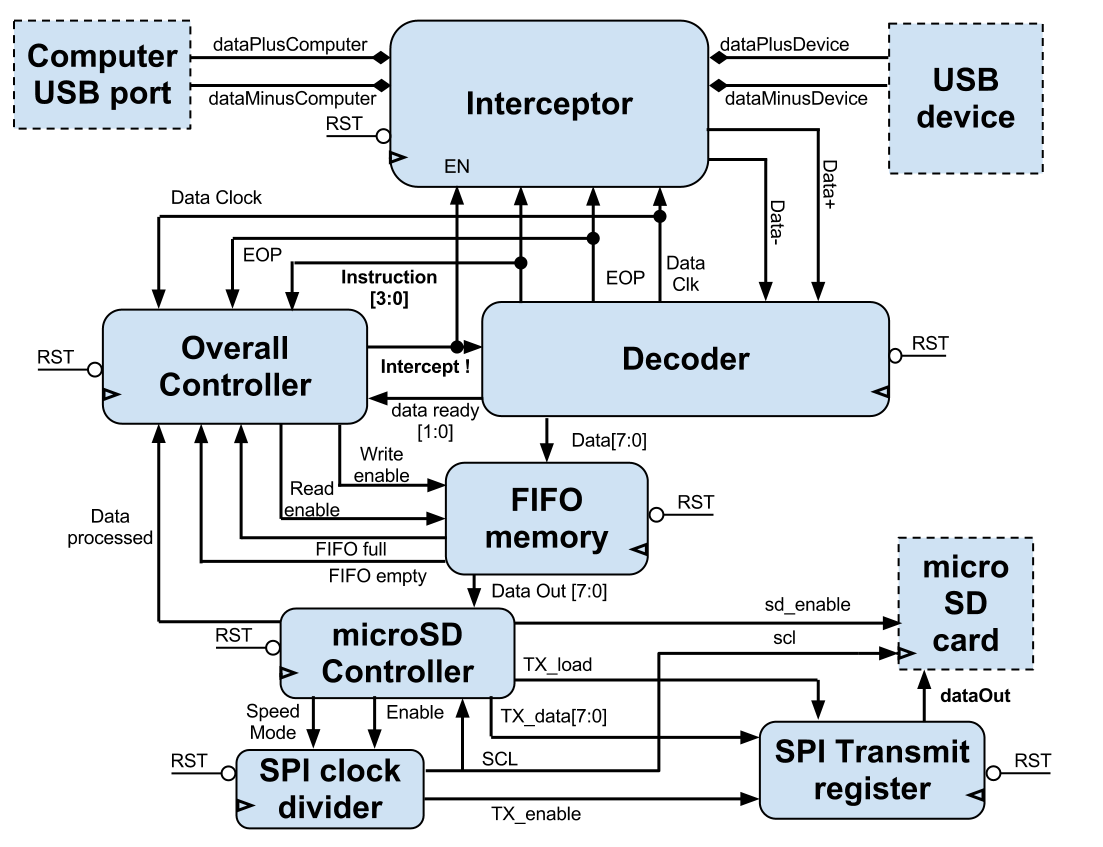
\includegraphics[width=0.95\textwidth]{topLevel}
	\end{center}
\end{figure}
\pagebreak
\section{Functional Block Diagrams}
%\begin{figure}[h]
%	\begin{minipage}[b]{0.5\linewidth}
%		\centering
%		\caption{The decoder's block diagram}
%		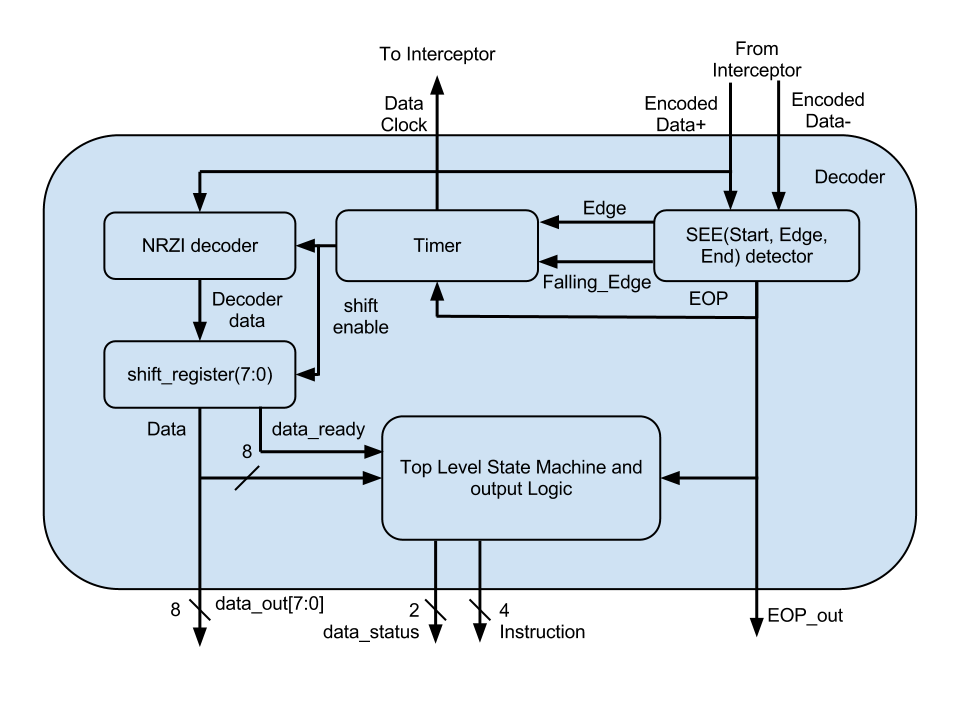
\includegraphics[width=0.98\textwidth]{decoderBlock}
%	\end{minipage}
%	\hspace{0.5cm}
%	\begin{minipage}[b]{0.5\linewidth}
%		\centering
%		\caption{The decoder's State Transition Diagram}
%		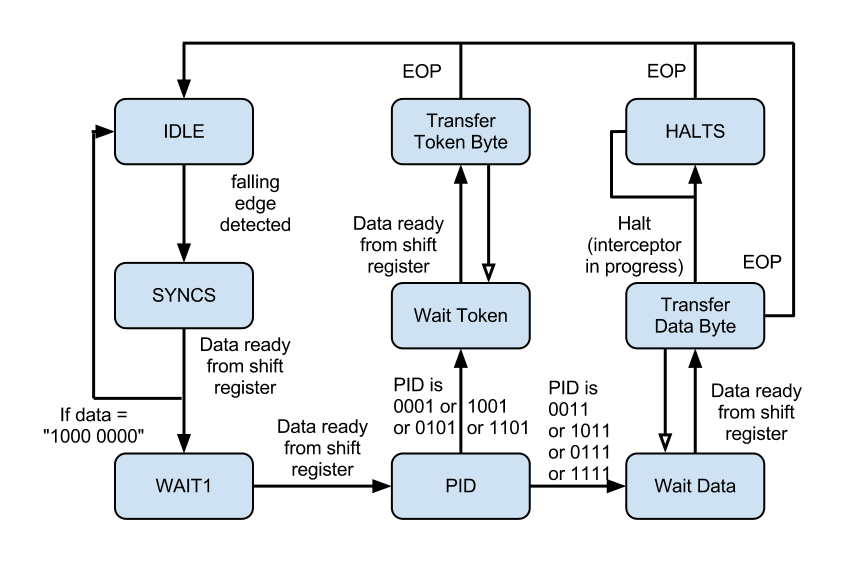
\includegraphics[width=0.98\textwidth]{decoderTrans}
%	\end{minipage}
%\end{figure}
\subsection{Controller}
\begin{figure}[h!]
	\centering
	\caption{The controller's state transition diagram}
	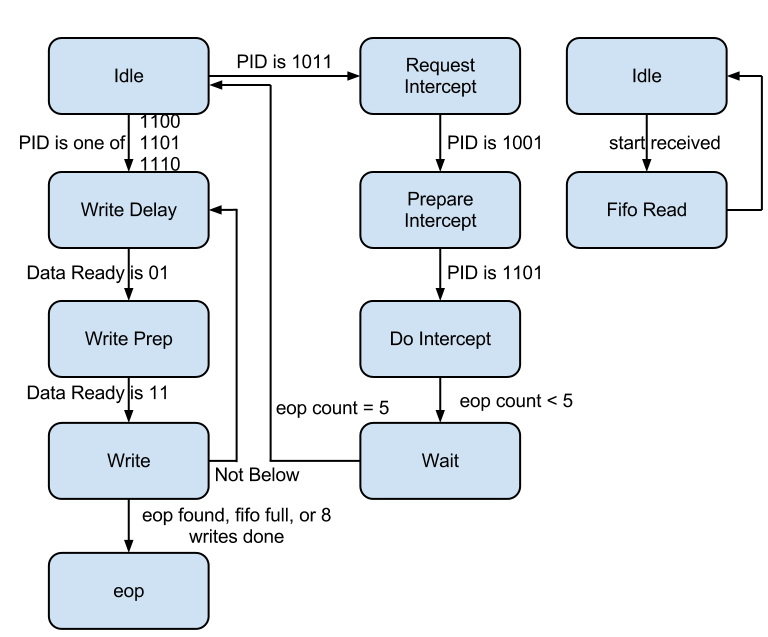
\includegraphics[width=0.75\textwidth]{controllerTrans}
\end{figure}
Here, the controller's state machines are featured. The Controller has two seperate state machines, one for controlling the USB read and one for controlling the microSD write. The USB data state machine is primarily a two-part machine: intercept, and read data. If the appropriate PID is found, it will tell the interceptor to do it's job, at which point the device descriptor packet will be appropriately modified. However, if a different set of PIDs is found, it will wait for the decoder to get a full byte and output it to the FIFO, as we are receiving data packets. It ignores all other PIDs, as we won't need to intercept or record in those cases.
\pagebreak
\subsection{Decoder}
\begin{figure}[h!]
		\centering
		\caption{The decoder's block diagram}
		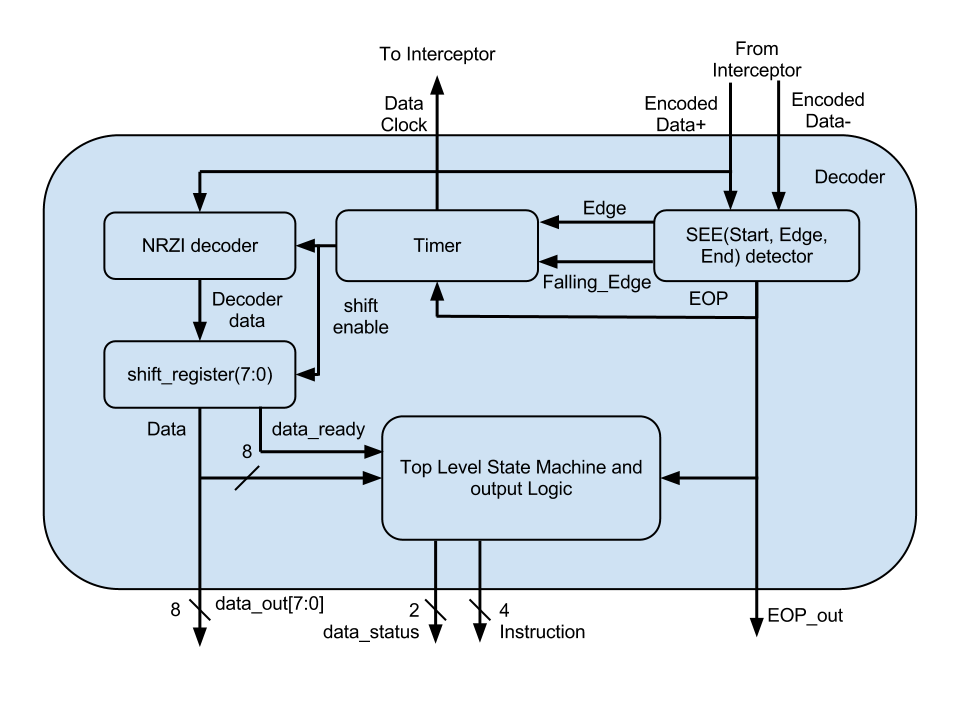
\includegraphics[width=0.75\textwidth]{decoderBlock}
\end{figure}
\begin{figure}[h!]
		\centering
		\caption{The decoder's state transition diagram}
		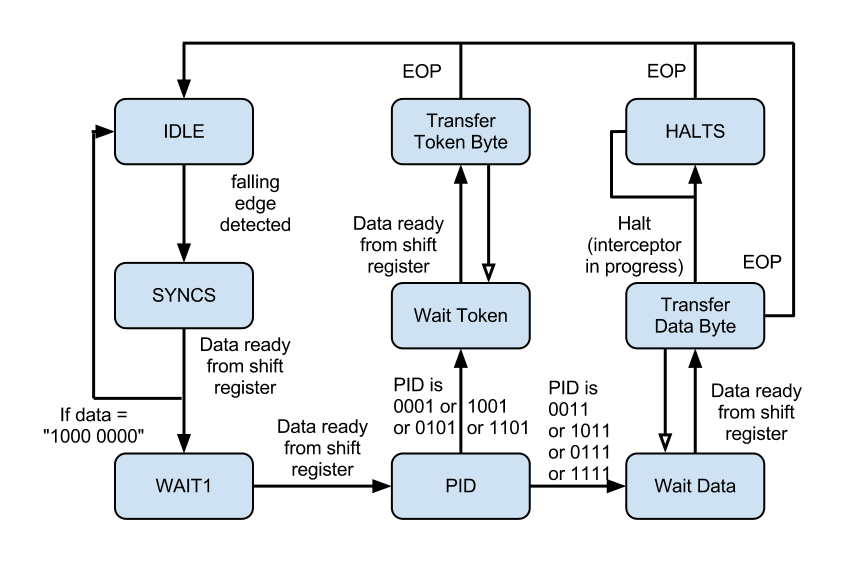
\includegraphics[width=0.75\textwidth]{decoderTrans}
\end{figure}
As you can see in figures 3.3 and 3.4, the decoder is primarily a state machine. The decoder also contains the timer, which is our data clock for USB, along with the SEE detector, which lets the other blocks know when an end of packet is on the line. The NRZI decoder recognizes and decodes the USB interface's non-return to zero, inverted signal and shifts in the appropriate bit to an internal shift register. When a full byte is loaded into the register, it outputs to the FIFO.
\subsection{Interceptor}
\begin{figure}[h!]
	\centering
	\caption{The interceptor's block diagram}
	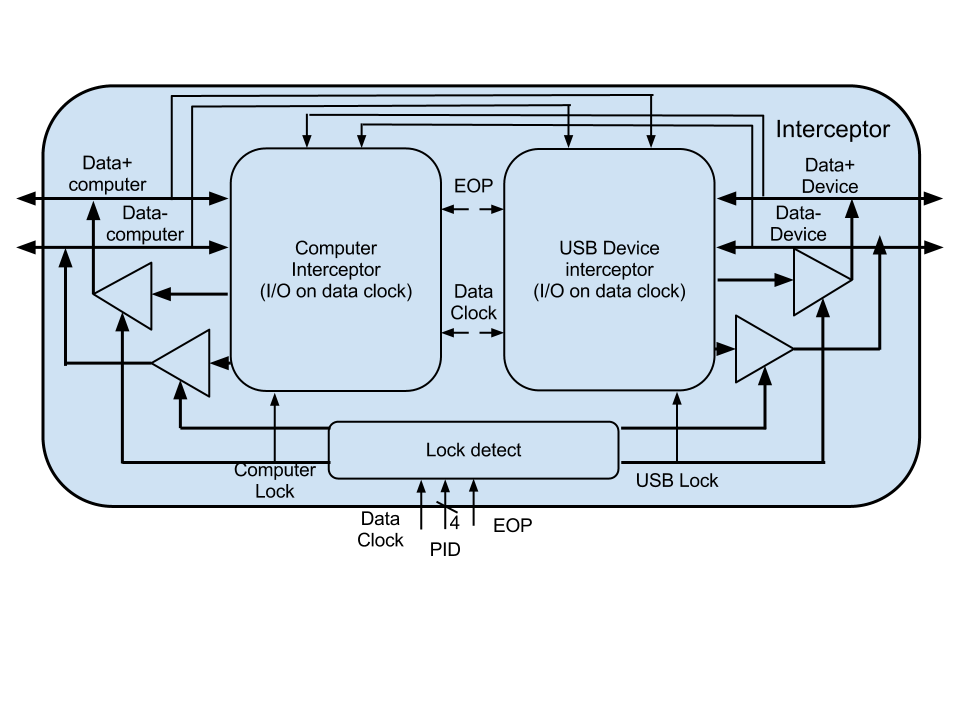
\includegraphics[width=0.75\textwidth]{interceptorBlock}
\end{figure}
\begin{figure}[h!]
	\centering
	\caption{The USB interceptor's state transition diagram}
	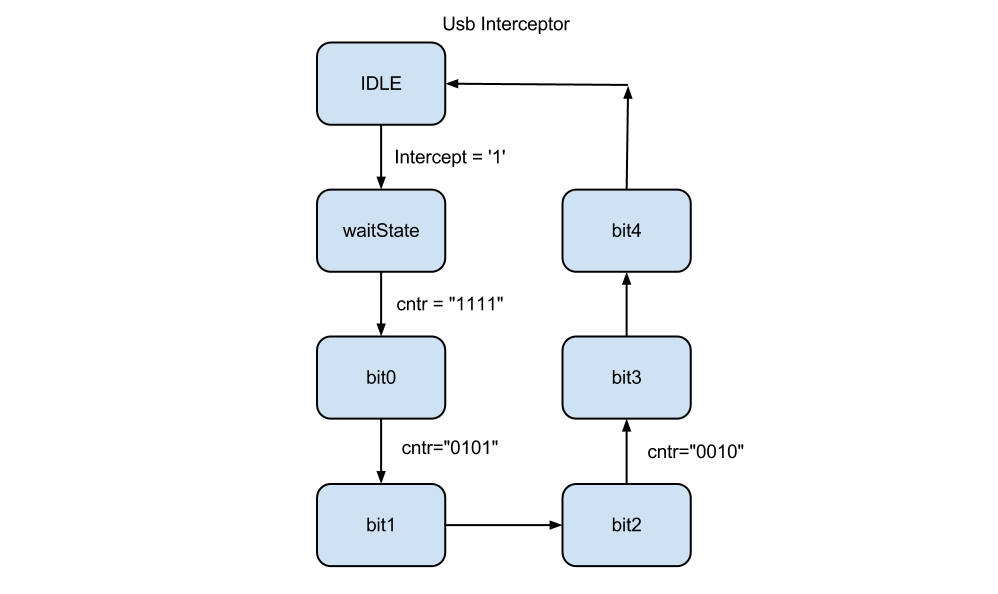
\includegraphics[width=0.75\textwidth]{interceptorTrans}
\end{figure}
In figures 3.5 and 3.6, we see the interceptor's block diagram and it's state machine. Again, this block is primarily a state machine. Normally, this block will simply be passing data through from one device to the other, with a slight delay. The "Lock detect" sub-block simply uses the PID from the token sent by the computer to decide which way data will be coming from. The "Computer Interceptor" sub-block simply passes through data, while the "USB Device Interceptor" sub-block actually does the intercepting, once it receives an intercept signal from the controller.
\pagebreak
\subsection{microSD Controller}
\begin{figure}[h!]
	\centering
	\caption{The microSD controller's block diagram}
	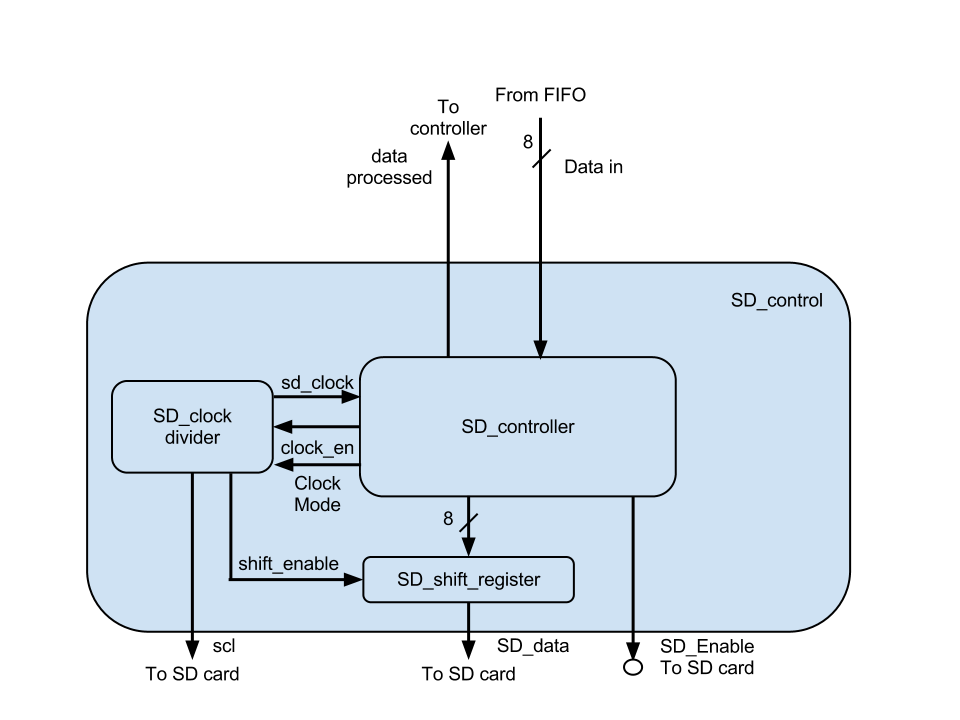
\includegraphics[width=0.70\textwidth]{sdBlock}
\end{figure}
Above, the SD controller block is shown. This block is relatively simple, despite what the state machine may have you believe. All this block does is initalize the SD card for writing, followed by writing data from the FIFO to the sd card. When the FIFO is empty, it will simply sit and wait for the FIFO to become non-empty, when it will begin it's outputting once more. It will continue in this loop infinitely.
\begin{figure}[h!]
	\centering
	\caption{The microSD controller's state transition diagram}
	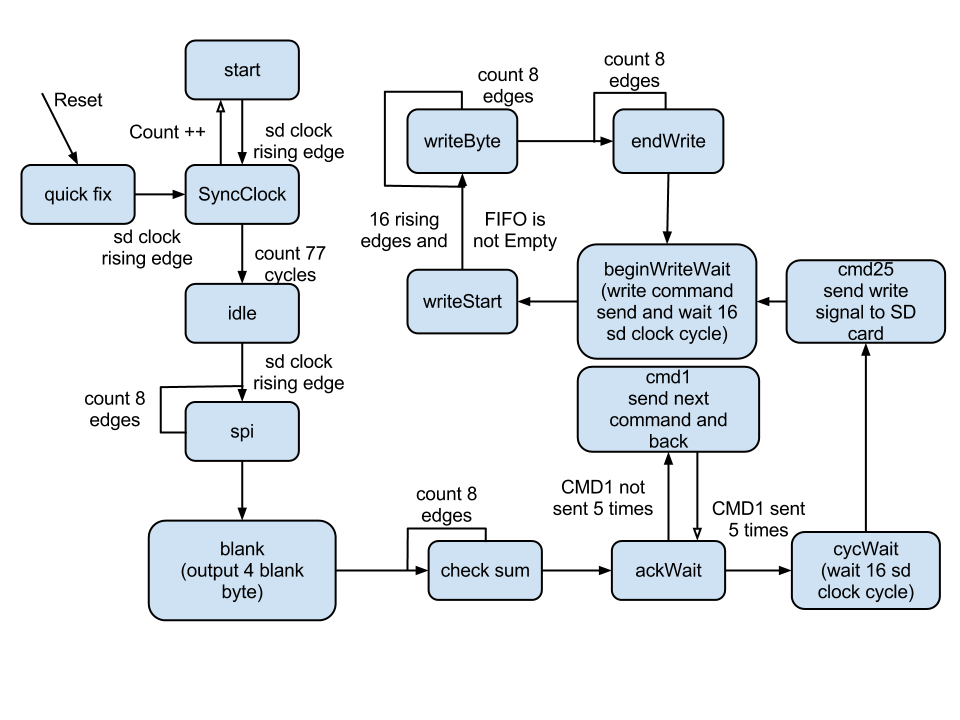
\includegraphics[width=0.73\textwidth]{sdTrans}
\end{figure}
\section{Standards and Protocols}
The USB Data Logger follows two protocols, USB 1.1 and SD via SPI. USB was chosen as it is currently the most widespread protocol used for communication between external devices and computers. USB 1.1 was specifically chosen due to it's significantly slower speed against USB 2.0 and USB 3.0. The .5 micrometer technology we are using is too slow to reach speeds faster than \SI{400}{\mega\hertz}. We would like to be at least 10x faster than the protocol we are following to allow for sufficient time to perform detection and manipulation of packets. As USB 2.0 is 480 Mbps, which is faster than even our fastest reasonably possible clocking speed, we were unable to use it as our protocol and decided on USB 1.1. \footnote{USB Protocol datasheet}

We chose microSD cards as an output device due to their small size and sufficient storage. After doing some research, the team was able to find microSD cards as large as 16 GB, which would be more than enough data to log keystrokes, mouse movements, or other low-data devices for several days, perhaps several weeks. \footnote{microSD datasheet 2} They could be used for some larger-data devices for a day or so. The size is sufficiently small such that, when the full device is manufactured, it would not need to be much bigger than the data logger ASIC. This allows for inconspicuous placing of the device with a low likelihood of being discovered.

Finally, we chose to communicate with the microSD card using SPI due to the simplicity and low pin count. SPI affords sufficient speed at a maximum of 50 Mbps, significantly faster than our clock and incredibly faster than USB 1.1, while still allowing us to write to the device using 3 lines for one-way communication and a simplified version of the SD protocol, allowing us to ignore CRC bits and checksums.

\section{Timing and Area Budgets}
\begin{table}[h]
	\caption{Timing and Area table}
	\centering
	\begin{tabular}{| l | l | l | l |}
		\hline
		& \bf{Critical Path} & \bf{Core Area} & \bf{Total Area} \\ \hline
		\bf{Success Critera} & \SI{7}{\nano\second} & Not Applicable & \SI{2.25}{\milli\meter\squared} \\ \hline
		\bf{Budget Assesment} & \multiline{\SI{4.3}{\nano\second} \\ Start: Sync Register \\ End: Controller \\ State Register} & \multiline{\SI{0.257}{\milli\meter\squared} \\ IO Pad Frame \\ Dimensions: \\ 870x\SI{870}{\micro\meter\squared} \\ IO Bounded} & \SI{1.97}{\milli\meter\squared} \\ \hline
		\bf{Design Compiler} & \multiline{\SI{1.78}{\nano\second} \\ Start: SD Control Register \\ End: SD Enable Output} & \SI{0.490}{\milli\meter\squared} & Not Applicable \\ \hline
		\bf{Encounter} & \SI{6.628}{\nano\second} & \SI{0.778}{\milli\meter\squared} & \SI{2.25}{\milli\meter\squared} \\ \hline
	\end{tabular}
\end{table}
According to table 3.1 on the previous page, the critical path delays and the area reports from the success criteria, budget assessment, design compiler, and encounter vary to a certain to degree. The reason for this could be caused by a number of factors, which may include changes to the design or the algorithms that encounter and design compiler use to calculate the paths and area.

Starting with the critical path delays, the chosen clock period was \SI{7}{\nano\second} (\SI{140}{\mega\hertz} clock speed) because the design needed to be clocked at least ten times faster than the USB clock. The total area, on the other hand, needed to meet a relatively small target area of \SI{2.25}{\milli\meter\squared} because the ASIC device must not be larger than the microSD.

When it came to the budget assessment, the largest combinational path had to be found in order to determine the critical path. It was discovered that the largest path started from a sync register, through combinational logic in the decoder block, then through the next state logic in the controller, and finally ended at the state registers in the controller. Given the timing estimates for 0.5 micron technology, the calculated critical path for the budget was \SI{4.3}{\nano\second}. The budgeted core area was calculated to be \SI{0.257}{\milli\meter\squared}, which was found by estimating the number of registers and combinational logic in each block. The budgeted total area was calculated to be \SI{1.97}{\milli\meter\squared}.

Once the design was working in source simulations, the mapped version of our top-level was created through Design Compiler. The reports after synthesis yielded a \SI{1.78}{\nano\second} critical path delay that started from SD Control Register, and ended at the SD enable output.The reason why the budgeted path was lower than the Design Compiler critical path might be because the budgeted estimate was generous and the design had been modified while coding and testing the source. It may be possible that a register was coded in between the expected critical path in the budget, thus reducing the delay. The estimated  core area was reported to be \SI{0.49}{\milli\meter\squared}, which is larger than the budgeted estimate. The reason for this is that the design needed more components than what was originally expected.

A layout was then created in Encounter after the mapped simulations were working. The timing report from Encounter showed that the critical path delay was \SI{6.628}{\nano\second}, which is higher than the budgeted and Design Compiler estimates. The reason for this change is probably due to how Encounter calculates the paths since more factors are included in the calculation such as wiring and fan in/out delays. Even though \SI{6.628}{\nano\second} is the largest critical path estimate and probably the most accurate, it still meets the timing requirement of \SI{7}{\nano\second} clock period. On the other hand, the core area from Encounter reported \SI{0.788}{\milli\meter\squared}, which is higher than the budgeted and Design Compiler estimates. In addition, the total area estimate from Encounter was \SI{2.25}{\milli\meter\squared}, which precisely matches the maximum target area. The total area, however, is slightly larger than the calculated total area from the budget report, which was \SI{1.97}{\milli\meter\squared}. The reason for this might be caused by the number of components that were added to the design. Despite this, the design is able to meet the total target area of \SI{2.25}{\milli\meter\squared}.

The critical path delay of our design was able to meet its target of \SI{7}{\nano\second} with a \SI{6.628}{\nano\second} delay. The core area, however, was larger than what was originally anticipated even though our total area was able to meet its target. Attempts were made to try and reduce the core area from \SI{0.788}{\milli\meter\squared} down to \SI{0.257}{\milli\meter\squared}. The number of registers in the FIFO was one of the major causes of the problem. The design originally had twelve registers in the FIFO, and each register stored eight bits of data, which took up large amounts of area according to Design Compiler. Therefore, the FIFO size was decreased to a reasonable size with a reasonable amount of area. In addition, an effort was made to make the source code smaller and more efficient such as reducing the number of states in a FSM or removing signals that were not needed in the design.
\chapter{Testing}
The USB Data Logger was primarily tested against the design criteria, so additional tests could be performed to ensure proper functionality. Each primary sub-component of the top-level device was tested using it's own, independent test bench, however most of the sub-components were modified slightly when integrated with the full design. With that said, some of these sub-component test benches no longer work as well as they were originally intended.

The ASIC was designed to handle two different operations that can occur separately or simultaneously. One part of the ASIC is the interceptor, decoder, and overall controller, which handles the USB protocol injection and data extraction. The other half of the ASIC is the SD Controller, FIFO, clock divider, and transmit shift register, which handles the clock, enable, and data signals that go to the micro SD. The test bench had to be made to test both of these processes working separately and at the same time. The test bench for the design utilizes a USB packet record, a NRZI encoding function, and several procedures to accurately simulate the transactions on a USB bus, and to make the design testing process simpler.

The record is composed of the different fields that any packet sent on the bus can have. These fields include synchronize, PID, address, end point, data, and cycle redundancy check (5 and 16 bits depending on the packet). An end of packet field could have been part of the record, however both data lines should be pulled low during an end of packet. So, having an end of packet field did not seem necessary. In addition, test vectors were created to store data for each packet sent on the bus. Each field in the test vector corresponds to the attributes in the record.

The NRZI encoding function was used to encode the testing data bits in the test bench such that the bits on the USB bus would be NRZI encoded in the simulation. The function accepts the decoded data that is meant to be transmitted on the bus, and the value on the data line. If the decoded data is zero then the value on the data line is flipped, otherwise if the decoded data is one then the value on the data line stays the same. This function was simply meant for convience so that the test data would not have to be encoded, and can therefore be easily read and created.

Lastly, there were several procedures used in the test bench that are meant to send different USB packets on the bus. Each procedure uses the NRZI encoding function to encode the test data from the test bench, and if either the device or the host is driving the bus, then the D+ and D- lines of the component that is receiving the bits is pulled high and low, respectively. This is was done because tristates on a bi-directional bus require either pull-up or pull-down resistors, so that the bus never goes into a high impedance state. The first procedure simulates the token packet that is sent from the host. It is flexible enough to support any kind of token (Setup, In, Out, SOF), which is determined by the test vectors. This procedure sends the sync byte first followed by the PID, address, end point, crc5, and then the end of packet. After the end of packet is transmitted, the bus will go idle. The next two procedures simulate data transmissions from the device or the host. Both of these procedures send the sync byte first followed by the PID, data, crc16, and then transitions from the end of packet back to idle. The last two procedures simulate the ack from the device or the host. Both of these procedures send the sync byte first followed by the PID, and then transitions from the end of packet back to idle. The last procedure that was created simulates the transmission check packet. This packet is only used after the device description has been sent from the device. If the transaction was successful then the host will send a zero length packet, which basically means there is no data field. So, this procedure is similar to the data procedure mentioned earlier, however there the data field is left out.

    After creating the record, NRZI function, and procedures, the commands to run the test bench lie in the main process. This process was created to send packets using only one line of code with the help of the procedures. So, if the host wanted to know the device description of the device, then the test bench would be able to simulate those transactions in only a few lines of code. The necessary procedures would be called upon to send the appropriate packets.

The full design was tested using a small series of packets over a simulated USB data line. Among the seven tests, five of them were standard data packets to ensure proper reading and writing, with the remaining two used to ensure proper intercepting of USB 3.0 and USB 2.0 device descriptors. All seven tests were deemed successful. Each test case is listed below:

\begin{enumerate} \itemsep 1pt
	\item Intercept a USB 3.0 descriptor and replace with USB 1.1
	\item Intercept a USB 2.0 descriptor and replace with USB 1.1
	\item Data "0xdeadbeeffeedbeef" is sent from the device to the computer
	\item Data "0xaaabbbcccdddeeef" is sent from the device to the computer
	\item Data "0xfff9998887776665" is sent from the device to the computer
	\item Data "0x1010101010f00730" is sent from the device to the computer
	\item Data "0x1337933244881122" is sent from the computer to the device
\end{enumerate}

The first test case sends several packets between the host and the device, which can ultimately be divided into three steps and each step can be divided into three packets. The first step is for the host to request the USB description of the device. This step starts with the host sending the setup token, then the request description packet is sent, and then it ends with an ack fro the device. The second step is when the USB sends the device description, which starts with the host sending an in token, then the USB 3.0 device description is sent from the USB, and then it ends with an ack from the host. The third and final step is the transaction check, which starts with the host sending an out token, then the host sends a zero length data packet, and then it ends with an ack from the device. The second test case is very similar to this.

    Test cases three through six are data packets that are sent from the device to the host. The first packet is the in token which is sent from the host, then the device sends data to the host, and then it ends with an ack from the host. The last test case works in a similar way, however data is now being sent from the host to the device. The first packet is the out token which is sent from the host, then the host sends data to the device, and then it ends with an ack from the device. 
\chapter{Layout}
\begin{figure}[h]
	\caption{The layout of the USB Data Logger, as generated by Virtuoso and Encounter, respectively}
	\begin{center}
		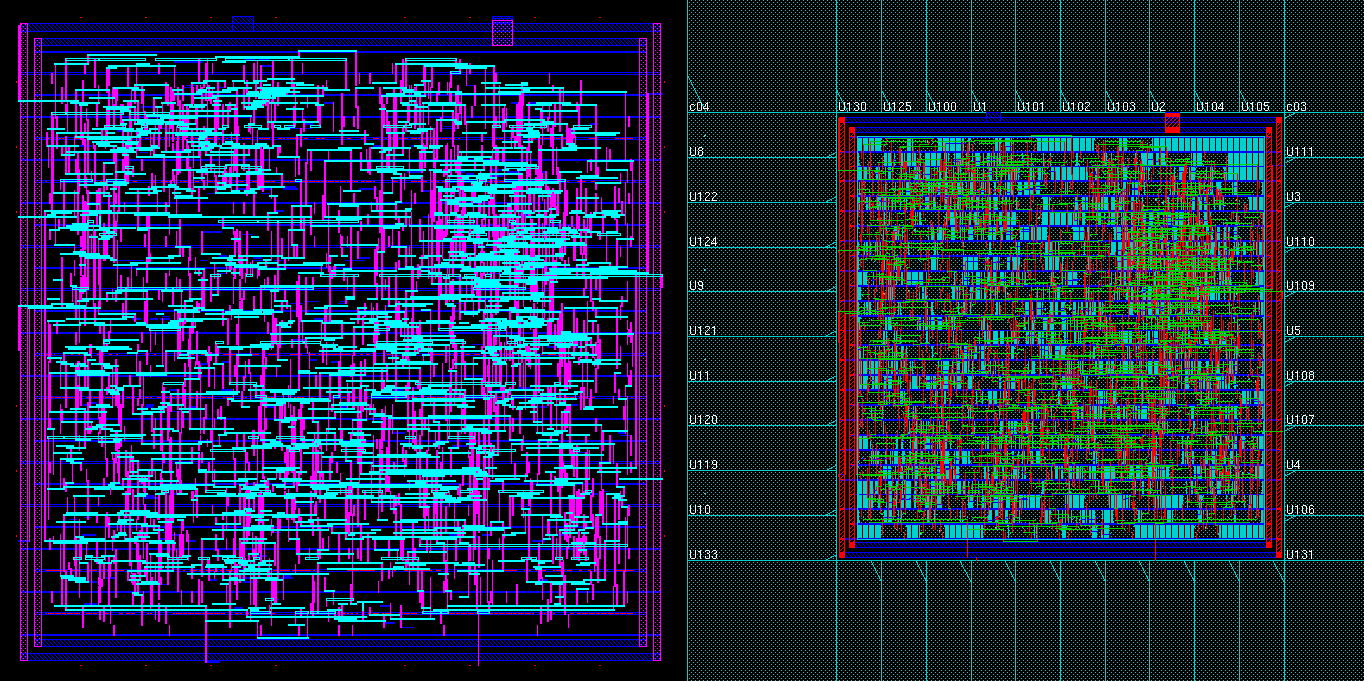
\includegraphics[width=0.95\textwidth]{virtuoso}
	\end{center}
\end{figure}
\begin{table}[h]
	\caption{Layout information provided by Encounter and Virtuoso}
	\centering
	\begin{tabular}{| l | l |}
		\hline
		\bf{Aspect Ratio} & 1.0 \\ \hline
		\bf{Row Utilization} &  1.8 \\ \hline
		\bf{Surrounding Area around Core (\si{\micro\meter})} & 40 \\ \hline
		\bf{Core Dimensions(\si{\micro\meter})} & 890 x 885 \\ \hline
		\bf{Core Area(\si{\milli\meter\squared})} & 0.787 \\ \hline
		\bf{Total Dimensions(\si{\micro\meter})} & 1500 x 1500 \\ \hline
		\bf{Total Area (\si{\milli\meter\squared})} & 2.25 \\ \hline
		\bf{Number of Gates} & 2337 \\ \hline
	\end{tabular}
\end{table}
\chapter{Results}
\section{Fixed Success Critera}
\begin{enumerate}
	\item Test benches exist for all top level components and the entire design. The test benches for the entire design can be demonstrated or documented to cover all of the functional requirements given in the design specific success criteria. \hfill \textbf{Result: Success}
	\item Entire design synthesizes completely, without any inferred latches, timing arcs, and, sensitivity  list warnings. \hfill \textbf{Result: Success}
	\item Source and mapped version of the complete design behave the same for all test cases. The mapped version simulates without timing errors except at time zero. \\ \vspace{-2.5em}\begin{flushright}\textbf{Result: Success}\end{flushright}
	\item A complete IC layout is produced that passes all geometry and connectivity checks. \\  \vspace{-2.5em}\begin{flushright}\textbf{Result: Success}\end{flushright}
	\item The entire design complies with targets for area, pin count, throughput (if applicable), and clock rate.  \hfill \textbf{Result: Success}
\end{enumerate}
\section{Design Specific Success Critera}
\begin{enumerate}
	\item Demonstrate by simulation of VHDL test benches that the complete design is able to correctly write data to the external SD card by attaching the SPI Master from the chip to an SPI Slave. \hfill \textbf{Result: Success}
	\item Demonstrate by simulation of VHDL test benches that the complete design is able to successfully remain transparent when intercepting data bits from the bus. \\ \vspace{-2.5em}\begin{flushright}\textbf{Result: Success}\end{flushright}
	\item Demonstrate by simulation of VHDL test benches that the complete design is able to correctly recognizes the default USB protocol handshake. \hfill \textbf{Result: Success}
	\item Demonstrate by simulation of VHDL test benches that the complete design is able to successfully modify the default USB protocol handshake into the USB 1.1 protocol and inject it into the USB bus \hfill \textbf{Result: Success}
\end{enumerate}
\appendix
\chapter{Data Sheets and Guide to Design Data}
\begin{description}
\item[Account and directory where all of the files are located:] \hfill mg56/ECE337/Project \\
 \begin{description}\itemsep0pt \parskip0pt \parsep0pt
   \item[Top level structural VHDL code] \hfill source/sniffer\_top.vhd \\
   \item[Computer Interceptor sub-component] \hfill source/computerInterceptor.vhd \\
   \item[Overall Controller] \hfill source/controller.vhd \\
   \item[Top Level Decoder] \hfill source/decoder.vhd \\
   \item[Fifo Ram sub-component] \hfill source/FifoRam.vhd \\
   \item[Fifo Read Pointer sub-component] \hfill source/FifoRead.vhd \\
   \item[Top Level Fifo] \hfill source/FifoTop.vhd \\
   \item[Fifo Write Pointer sub-component] \hfill source/FifoWrite.vhd \\
   \item[Top Level Interceptor] \hfill source/interceptor.vhd \\
   \item[Locking Detector sub-component]  \hfill source/lockingDetector.vhd \\
   \item[NRZI decoder sub-component] -\hfill source/NRZIdecode.vhd \\
   \item[SD Controller] \hfill source/sd\_control.vhd \\
   \item[Edge detector sub-component] \hfill source/SEE\_det.vhd \\
   \item[Shift Register sub-component] \hfill source/shift\_greg.vhd \\
   \item[Spi Clock Divider] \hfill source/SpiClkDivide.vhd \\
   \item[Spi Shift Register] \hfill source/SpiXmitSR.vhd \\
   \item[Timer sub-component] \hfill source/timer.vhd \\
   \item[Tristate sub-component] \hfill source/tristate.vhd \\
   \item[USB Interceptor sub-component] \hfill source/usbInterceptor.vhd \\
\end{description}


\item[Test Benches] \hfill \\
 \begin{description}\itemsep0pt \parskip0pt \parsep0pt

   \item[Sniffer Top Level test bench] \hfill source/tb\_sniffer\_top.vhd \\
   \item[Computer Interceptor test bench] \hfill source/tb\_computerInterceptor.vhd \\
   \item[Overall Controller test bench] \hfill source/tb\_controller.vhd \\
   \item[Fifo test bench] \hfill source/tb\_FifoTop.vhd \\
   \item[Interceptor test bench] \hfill source/tb\_interceptor.vhd \\
   \item[SD Controller test bench] \hfill source/tb\_sd\_control.vhd \\
   \item[Spi Clock Divide test bench] \hfill source/tb\_SpiClkDivide.vhd \\
   \item[Spi Transmit Shift Register test bench] \hfill source/tb\_SpiXmitSR.vhd \\
   \item[Tristate test bench] \hfill source/tb\_tristate.vhd \\
   \item[USB Interceptor test bench] \hfill source/tb\_usbInterceptor.vhd \\
\end{description}

\item[Report Files] \hfill
 \begin{description}\itemsep0pt \parskip0pt \parsep0pt

   \item[Sniffer Top Level Design Compiler Report] \hfill reports/sniffer\_top.rep \\    \item[Sniffer Top Level Encounter Report] timingReports/sniffer\_top\_postRoute\_all.tarpt \\
\end{description}

\item[Scripts] \hfill
 \begin{description}\itemsep0pt \parskip0pt \parsep0pt

   \item[Sniffer Top Level Script] \hfill scripts/sniffer\_top.fcr \\
\end{description}

\item[Presentation] \hfill
 \begin{description}\itemsep0pt \parskip0pt \parsep0pt

   \item[ECE 337 Final Presentation] \hfill docs/337FinalPresentation.pdf \\
\end{description}
\pagebreak
\item[Final Report] \hfill
 \begin{description}\itemsep0pt \parskip0pt \parsep0pt
  \item[Final Report Document] \hfill docs/finalReport/finalReport.pdf \\
  \item[Final Report LaTeX File] \hfill docs/finalReport/finalReport.tex \\
  \item[Title Page LaTeX File] \hfill docs/finalReport/titlePage.tex \\
  \item[Appendix A LaTeX File] \hfill docs/finalReport/appendixa.tex \\
  \item[Table of Contents] \hfill docs/finalReport/finalReport.toc \\
  \item[LaTeX Log File] \hfill docs/finalReport/finalReport.log \\
  \item[LaTeX Aux File] \hfill docs/finalReport/finalReport.aux \\
  \item[Controller Transition Diagram] \hfill docs/finalReport/controllerTrans.png \\
  \item[Decoder Block Diagram] \hfill docs/finalReport/decoderBlock.png \\
  \item[Decoder Transition Diagram] \hfill docs/finalReport/decoderTrans.png \\
  \item[Encounter-generated Layout] \hfill docs/finalReport/encounter.png \\
  \item[Interceptor Block Diagram] \hfill docs/finalReport/interceptorBlock.png \\
  \item[Interceptor Transition Diagram] \hfill docs/finalReport/interceptorTrans.png \\
  \item[Operational Timeline] \hfill docs/finalReport/OperationalTimeline.png \\
  \item[microSD Output Testbench Diagram] \hfill docs/finalReport/outputToMicroSD.png \\
  \item[microSD Controller Block Diagram] \hfill docs/finalReport/sdBlock.png \\
  \item[microSD Controller Transition Diagram] \hfill docs/finalReport/sdTrans.png \\
  \item[Token Recognition Testbench Diagram] \hfill docs/finalReport/tokenRecognition.png \\
  \item[Design Architecture Diagram] \hfill docs/finalReport/topLevel.png \\
  \item[Transparency Testbench Diagram] \hfill docs/finalReport/transparency.png \\
  \item[System Usage Diagram] \hfill docs/finalReport/usageDiagram.png \\
  \item[USB 2.0 to USB 1.1 Testbench Diagram] \hfill docs/finalReport/usb2.png \\
  \item[USB 3.0 to USB 1.1 Testbench Diagram] \hfill docs/finalReport/usb3.png \\
  \item[Virtuoso and Encounter layout] \hfill docs/finalReport/virtuoso.png \\ 
\end{description}


\item[Datasheets] \hfill
 \begin{description}\itemsep0pt \parskip0pt \parsep0pt

   \item[ECE 337 USB Lab Manual] \hfill doc/lab6\_sp09.pdf \\
   \item[ECE 337 USB Slides] \hfill doc/Lab6\_USB.pdf \\
   \item[microSD datasheet 1] \hfill doc/Lattice\_microSD\_specs.pdf \\
   \item[microSD datasheet 2] \hfill doc/sandisk\_secure\_digital\_card.pdf \\
   \item[SPI Protocol datasheet] \hfill doc/SPI\_Protocol.pdf \\
   \item[USB Protocol datasheet] \hfill doc/USBProtocol.pdf \\
\end{description}

\end{description}

\chapter{Simulation Results}
\section{Token Identification}
\begin{figure}[h!]
	\centering
	\caption{Testbench showing identification of a USB Data Descriptor Token}
	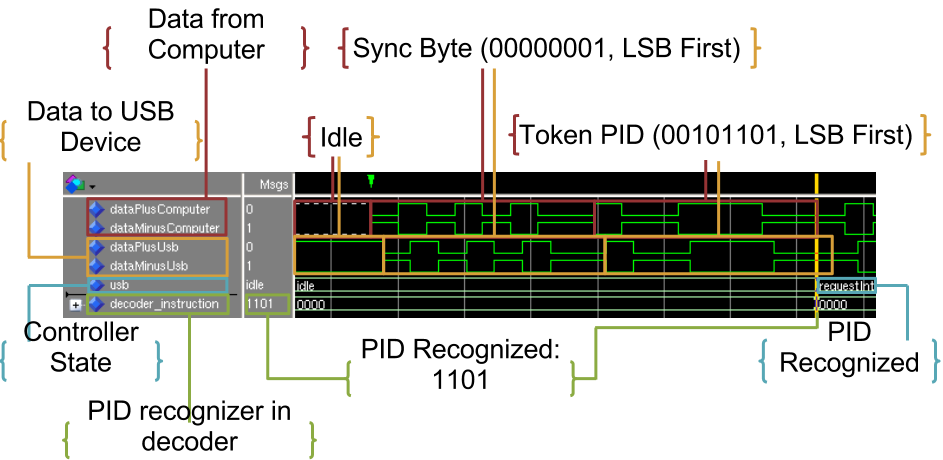
\includegraphics[width=.98\textwidth]{tokenRecognition}
\end{figure}
In figure B.1, the depicted testbench shows more than just the output signals. This must be done in order to show proper identification of a USB Data Descriptor Token. The top four lines are the data lines, identified using red and yellow, and are effectively identical for this test. After coming off of idle, the lines send a sync, followed by a PID, and ultimately followed by the appropriate data. You can see in the green decoder\_instruction line when the PID is recognized by the decoder, followed by when it is recognized by the controller on the blue USB line. 
\pagebreak
\section{Data Descriptor Modifications}
\subsection{USB 2.0 to USB 1.1}
\begin{figure}[h!]
	\centering
	\caption{USB 2.0 Data Descriptor Modification Testbench}
	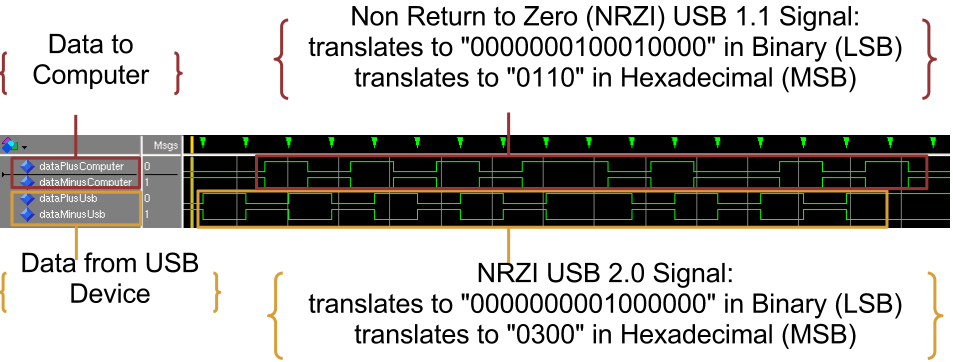
\includegraphics[width=.98\textwidth]{usb2}
\end{figure}
In figure B.2, we see the Data Descriptor being modified from USB 2.0 to USB 1.1. As you can see in the lower pair of lines, the data coming from the USB device is USB 2.0, 0x0200 (remember it is read least significant bit first). However, in the upper pair of lines, the data going to the USB device is USB 1.1, 0x0110.
\pagebreak
\subsection{USB 3.0 to USB 1.1}
\begin{figure}[h!]
	\centering
	\caption{USB 3.0 Data Descriptor Modification Testbench}
	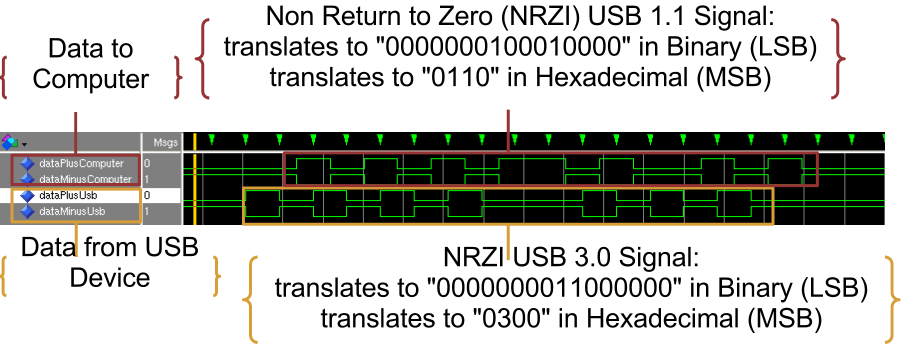
\includegraphics[width=.98\textwidth]{usb3}
\end{figure}
In figure B.3, we see a nearly identical test case to figure B.1, except that the modifcation is from USB 3.0 to USB 1.1. Notice that in the 2.0 test bench the NRZI encoding is reversed between lines until the end of packet, but in the 3.0 test bench this is not the case. That is because the binary reprsentations of the USB 3.0 and USB 1.1 descriptors (0x0300 and 0x0110 in hexadecimal) both have two ones, while the USB 2.0 descriptor (0x0200) only has one. After modifying this bit, we can't simply "follow" the bus directly anymore, but rather we have to look for changes between the lines and make our output match.
\pagebreak
\section{Transparency}
\begin{figure}[h!]
	\centering
	\caption{Testbench showing transparency between devices}
	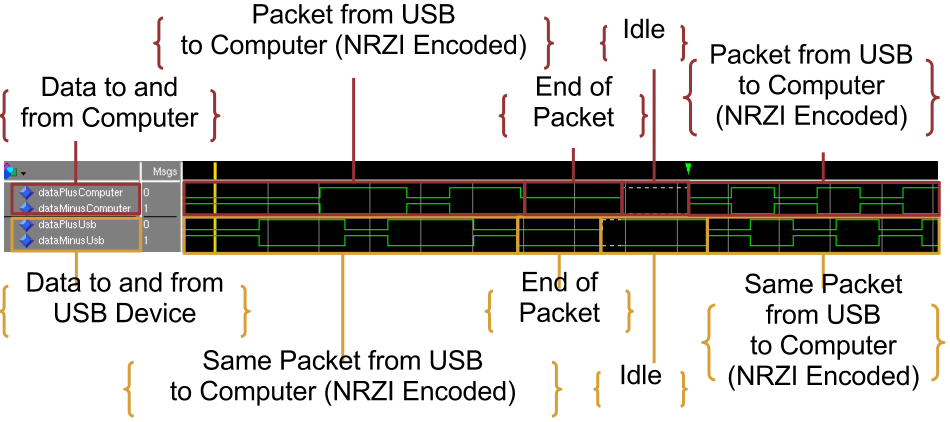
\includegraphics[width=.98\textwidth]{transparency}
\end{figure}
In figure B.4, we can see that data coming in from the USB device is identical to data going out to the computer before the end of packet. After the idle state, we can see the data coming in from the computer is identical to the data going out to the USB device.
\pagebreak
\section{microSD Output}
\begin{figure}[h!]
	\centering
	\caption{microSD card output}
	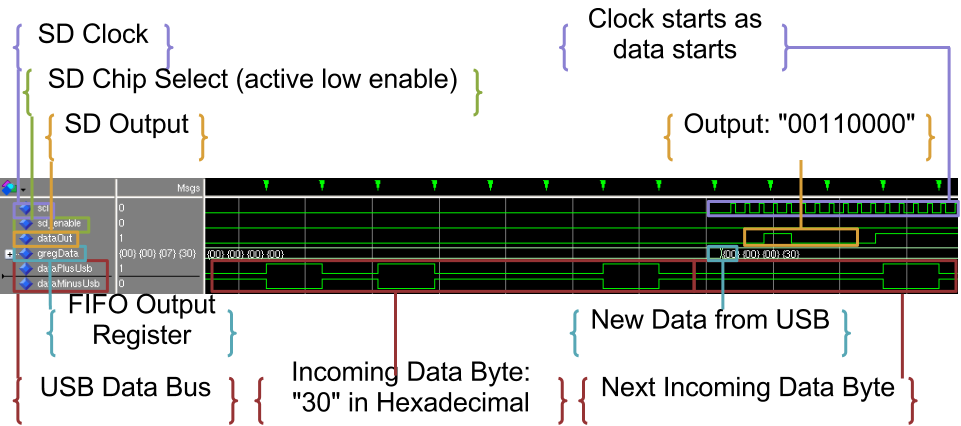
\includegraphics[width=.98\textwidth]{outputToMicroSD}
\end{figure}
In figure B.5, we can see the input from the USB device is 0x30. We see that this changes on the FIFO in the blue-labeled line, directly above it. When this happens, the SD Clock starts ticking, and it outputs the data from the device to the SD card. It continues to tick after the fact as it has to write a few commands to the SD card before it can continue.
\end{document}
